\section{Accesso alla piattaforma}\label{Accesso}
All'accesso della piattaforma l'utente visualizza la schermata principale contenente:
\begin{enumerate}
	\item Descrizione dell'azienda;
	\item Prodotti in evidenza;
	\item Barra per la ricerca dei prodotti;
	\item \glo{Icona} del menù.
\end{enumerate} 
\begin{figure}[H]
	\centering
	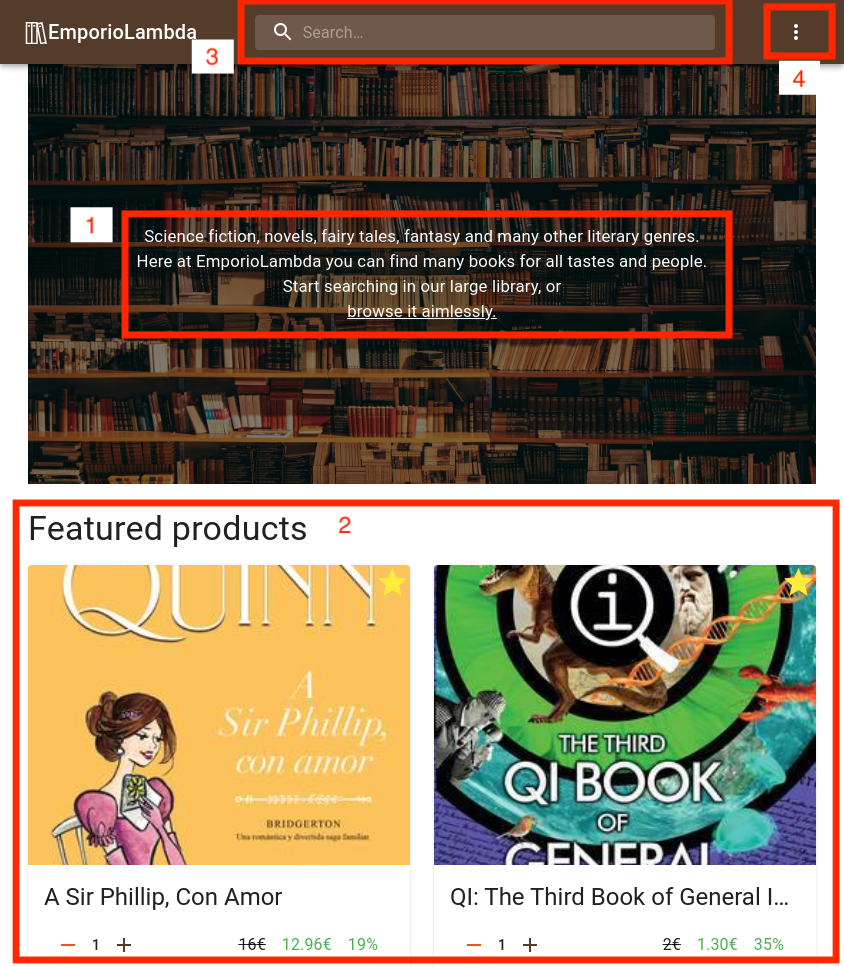
\includegraphics[scale=0.4]{Immagini/Acquirente/home_primo_accesso.png}
	\caption{Schermata principale}
	\label{fig:Home}
\end{figure}
Cliccando sull'icona del menù (4) appariranno due icone cliccabili dall'utente per poter visualizzare il proprio carrello o effettuare il login/registrazione.
\begin{figure}[H]
	\centering
	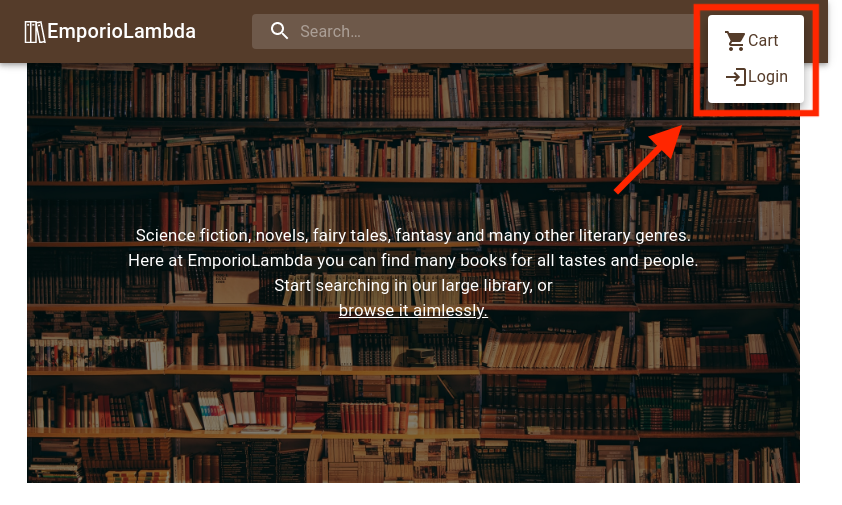
\includegraphics[scale=0.4]{Immagini/Acquirente/home-mobile-open.customer.png}
	\caption{Schermata principale con menù a tendina}
	\label{fig:Homeicone}
\end{figure}
\begin{figure}[h!]
	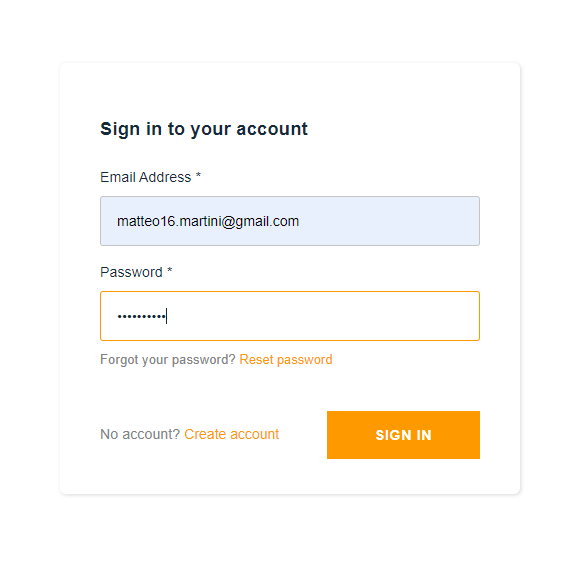
\includegraphics[scale=0.7]{Immagini/Acquirente/login.png}\quad
	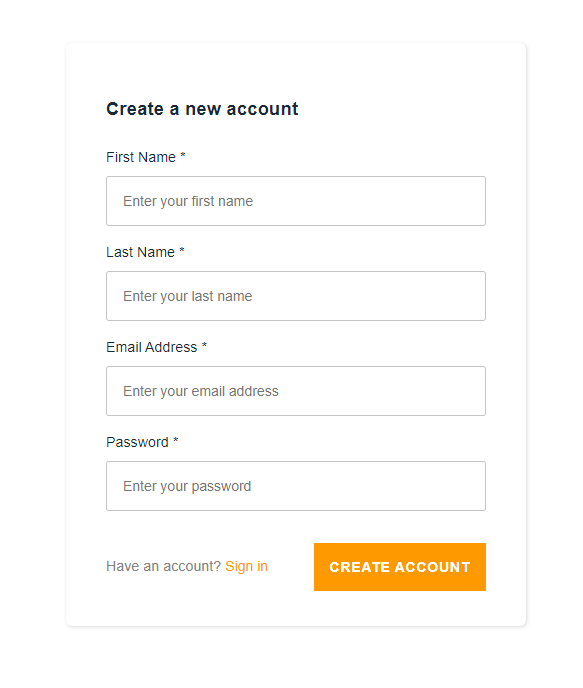
\includegraphics[scale=0.6]{Immagini/Acquirente/createAccount.png}
\end{figure}
\newpage
\section{Acquirente}\label{Acquirente}
La schermata principale visualizzata comprende nuovamente descrizione dell'azienda, prodotti in evidenza e:
\begin{enumerate}
	\item \glo{Icona} per accedere al carrello;
	\item Icona per effettuare il logout.
\end{enumerate} 
\begin{figure}[H]
	\centering
	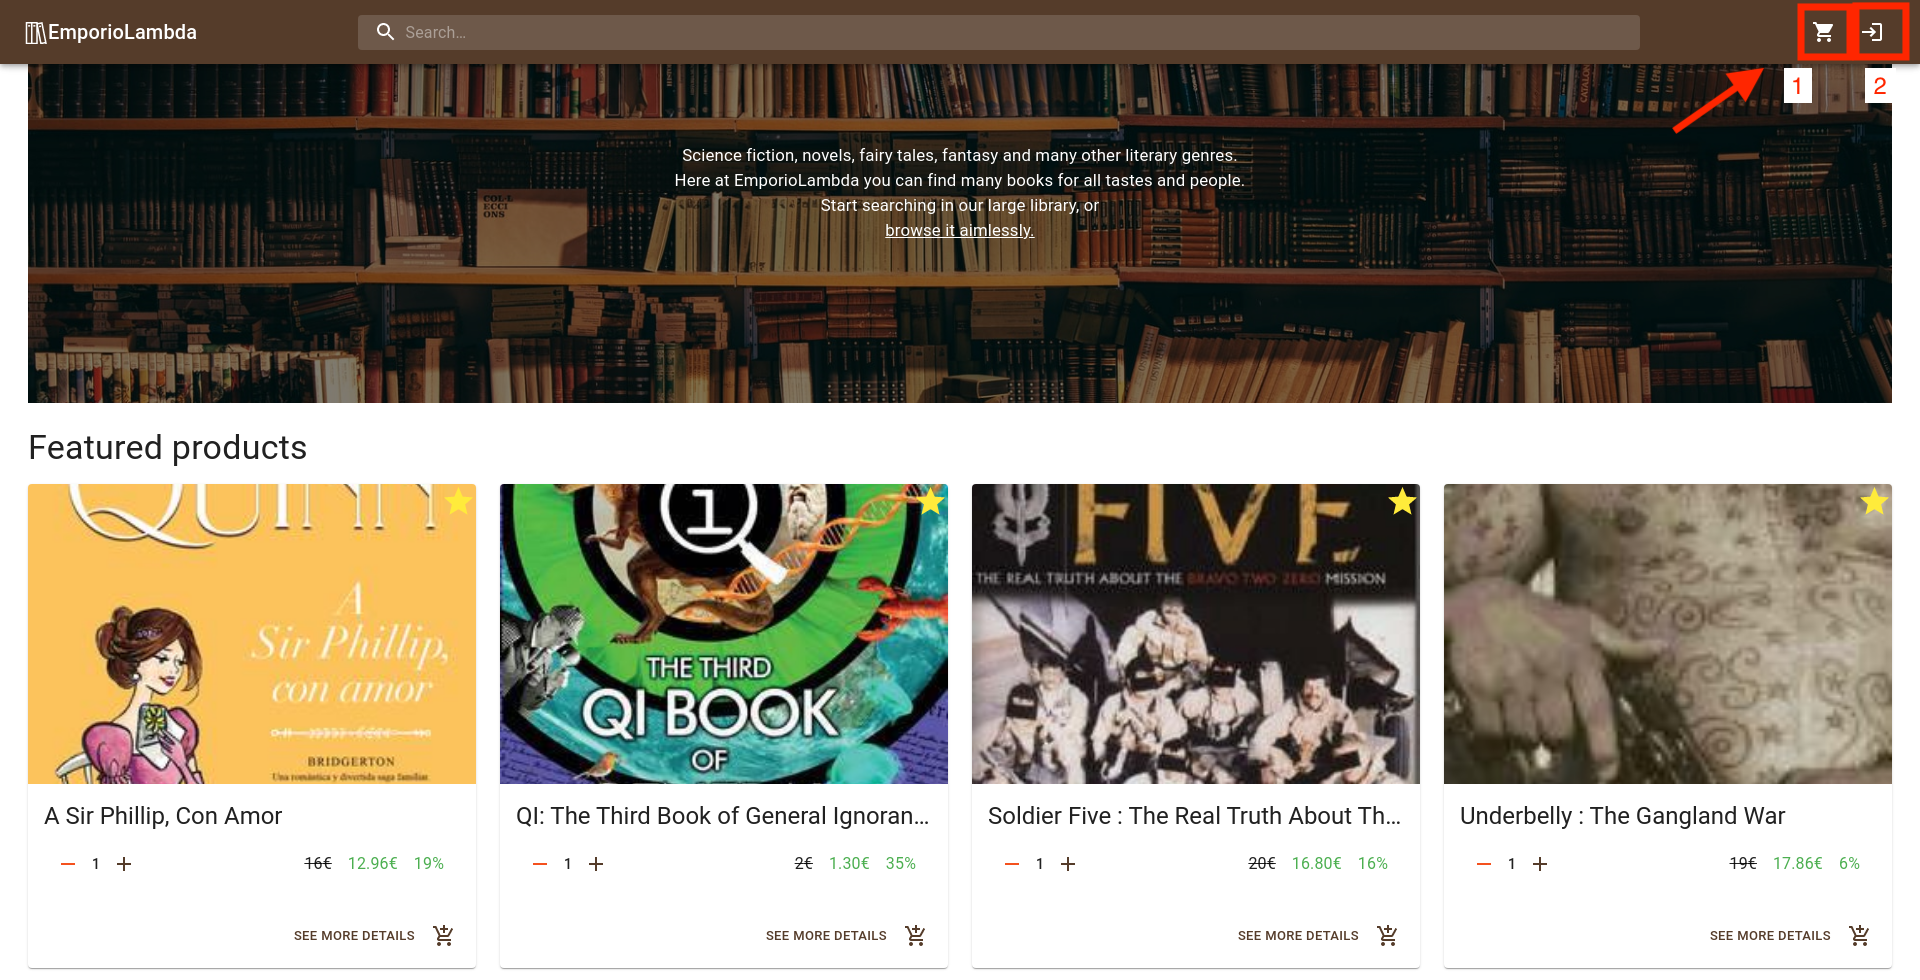
\includegraphics[scale=0.25]{Immagini/Acquirente/home.customer.png}
	\caption{Schermata principale utente autenticato}
	\label{fig:Homecustomer}
\end{figure}
\subsection{Visualizzazione specifiche di un prodotto}
L'acquirente, autenticato sulla piattaforma o come ospite, può visualizzare le specifiche di un prodotto in evidenza cliccando sullo stesso. La schermata alla quale sarà indirizzato comprenderà:
\begin{enumerate}
	\item Nome del prodotto;
	\item Elenco di immagini visualizzabili;
	\item Descrizione del prodotto;
	\item Prezzo ed eventuali sconti percentuali applicati;
	\item Categorie di appartenenza;
	\item Icone per modificare la quantità da inserire nel carrello e per inserire i prodotti nel carrello.
\end{enumerate} 
\begin{figure}[H]
	\centering
	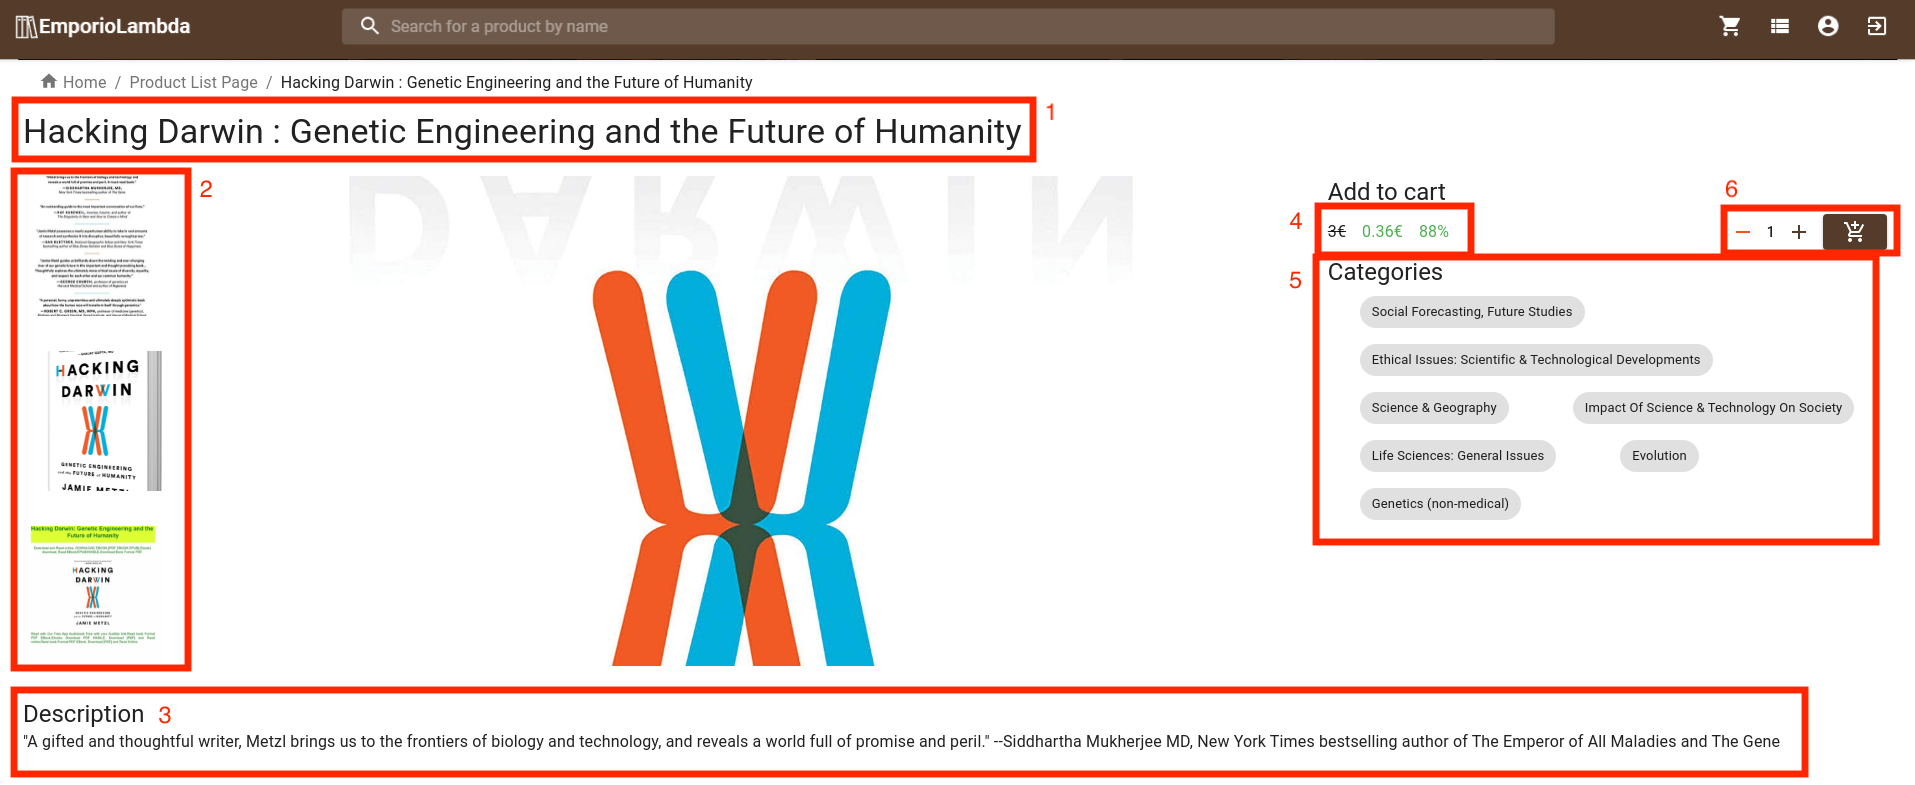
\includegraphics[scale=0.25]{Immagini/Acquirente/pdp.customer.png}
	\caption{Specifiche di un prodotto}
	\label{fig:SpecificheProdotto}
\end{figure}
\subsection{Visualizzazione elenco prodotti}
L'utente può visualizzare l'intero elenco di prodotti presenti nella piattaforma, per ognuno di essi sarà visualizzato nome, prezzo ed eventuali sconti, icone per modificare il numero di prodotti da inserire nel carrello e per inserire la quantità nel carrello. I prodotti non disponibili avranno un'indicazione sopra l'immagine del prodotto.
\begin{figure}[H]
	\centering
	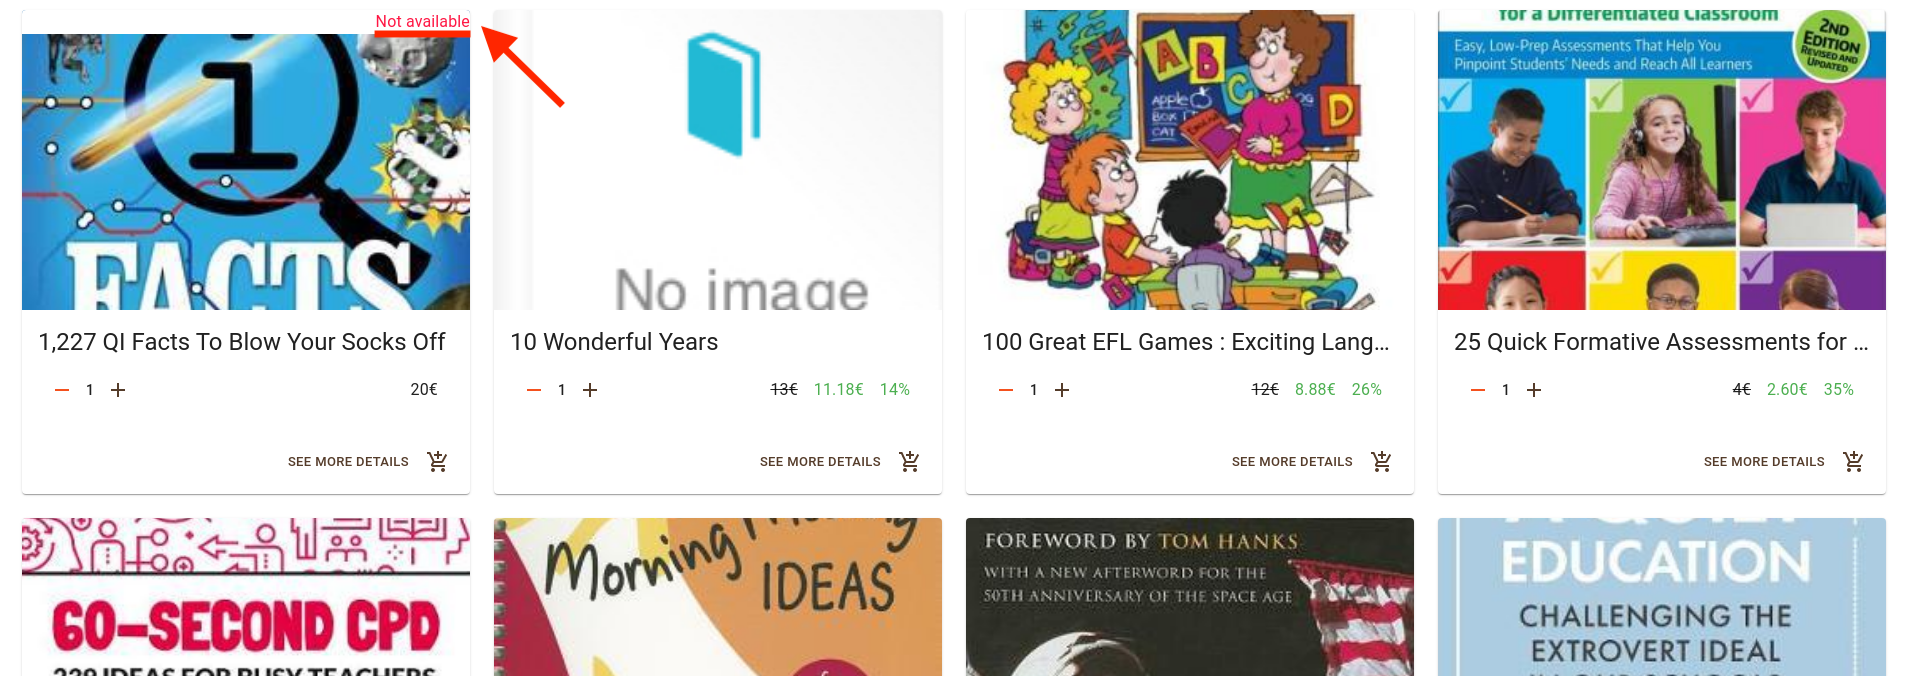
\includegraphics[scale=0.25]{Immagini/Acquirente/plp-pagination.customer.png}
	\caption{Schermata dei prodotti nella piattaforma}
	\label{fig:PLP}
\end{figure}
I prodotti possono essere visualizzati secondo un preciso ordine cliccando sull'apposita icona e selezionando il tipo di ordinamento desiderato.
\begin{figure}[H]
	\centering
	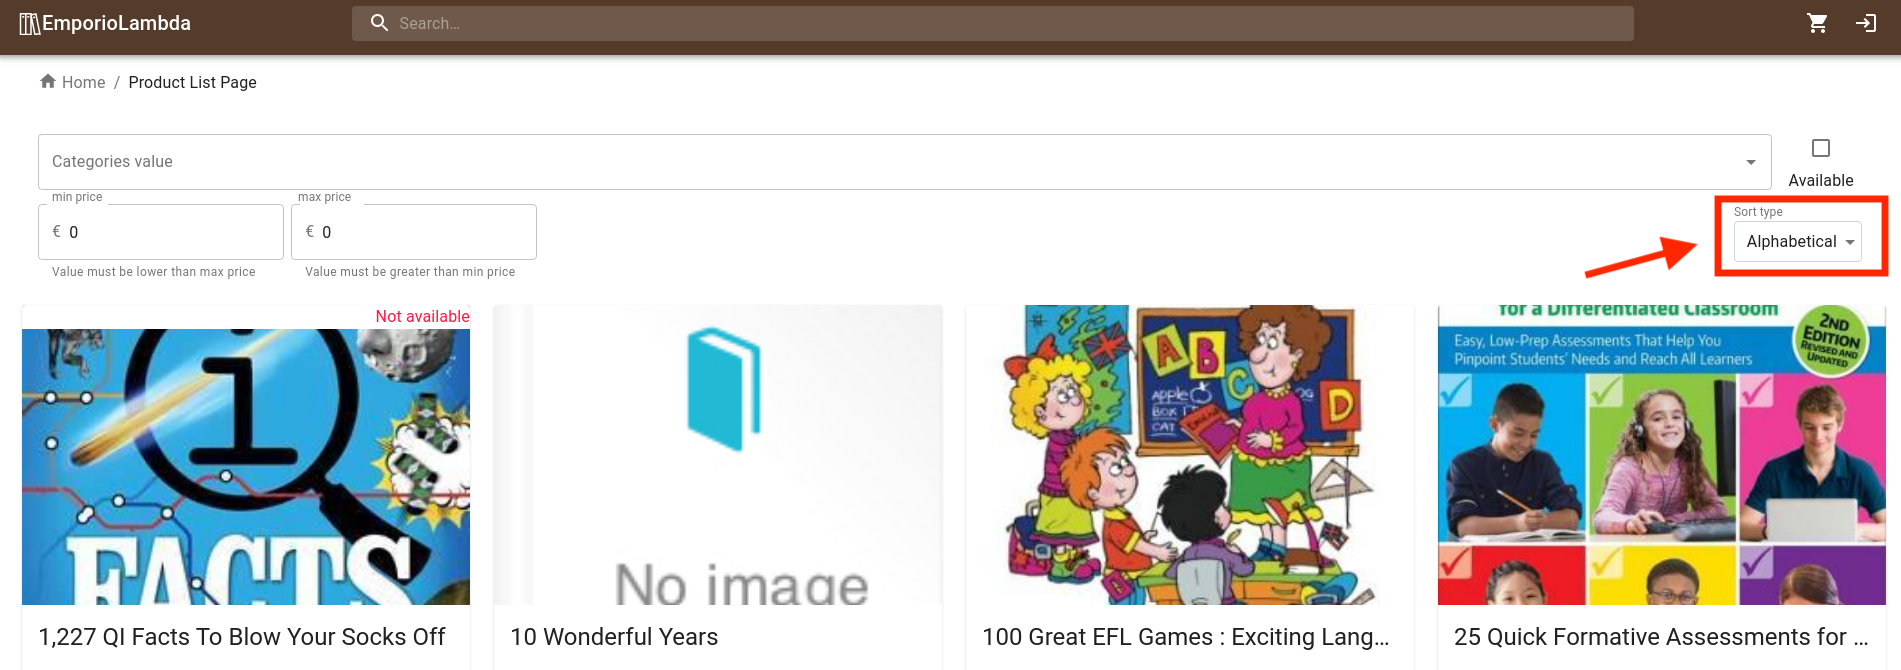
\includegraphics[scale=0.25]{Immagini/Acquirente/plp-sort1.png}
	\caption{Schermata dei prodotti nella piattaforma con ordinamento}
	\label{fig:PLPordinamento1}
\end{figure}
\begin{figure}[H]
	\centering
	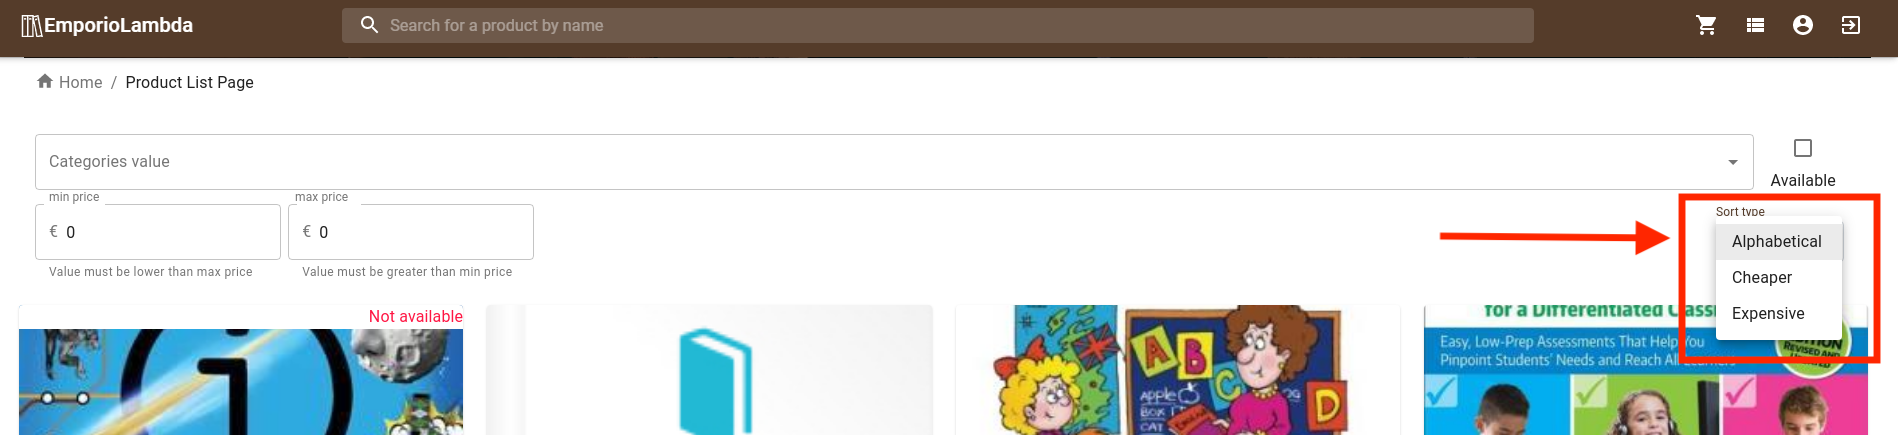
\includegraphics[scale=0.25]{Immagini/Acquirente/plp-sort-filter.png}
	\caption{Schermata dei prodotti nella piattaforma con possibili ordinamenti}
	\label{fig:PLPordinamento2}
\end{figure}
\subsection{Filtraggio dei prodotti}
Nella schermata con l'elenco prodotti l'utente può procedere a raffinare la sua ricerca impostando una serie di filtri.
\begin{figure}[H]
	\centering
	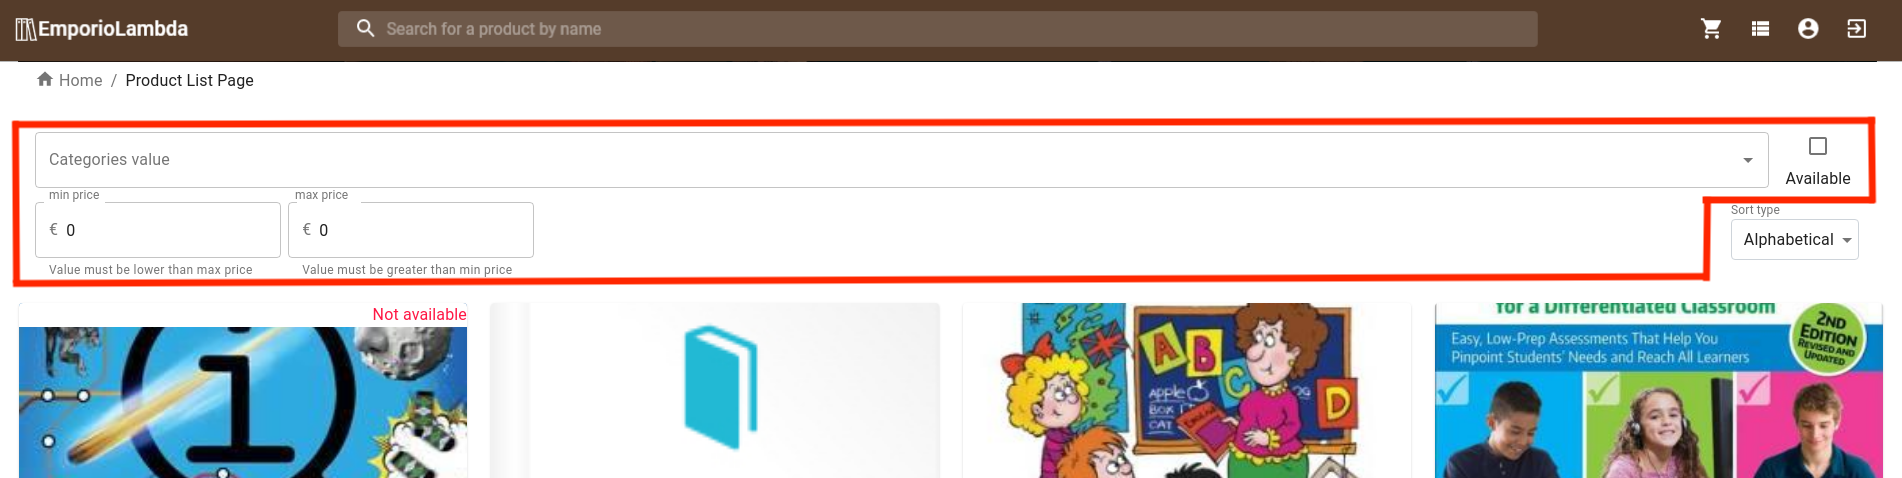
\includegraphics[scale=0.25]{Immagini/Acquirente/plp-filter.customer.png}
	\caption{Schermata dei prodotti con filtri applicabili}
	\label{fig:PLPfiltri}
\end{figure}
\subsubsection{Filtro prodotti per categorie}
Per ricercare un prodotto in base alle categorie di appartenenza, l'utente può cliccare sulla prima barra di ricerca e selezionare le categorie di interesse tra quelle visualizzate.
\begin{figure}[H]
	\centering
	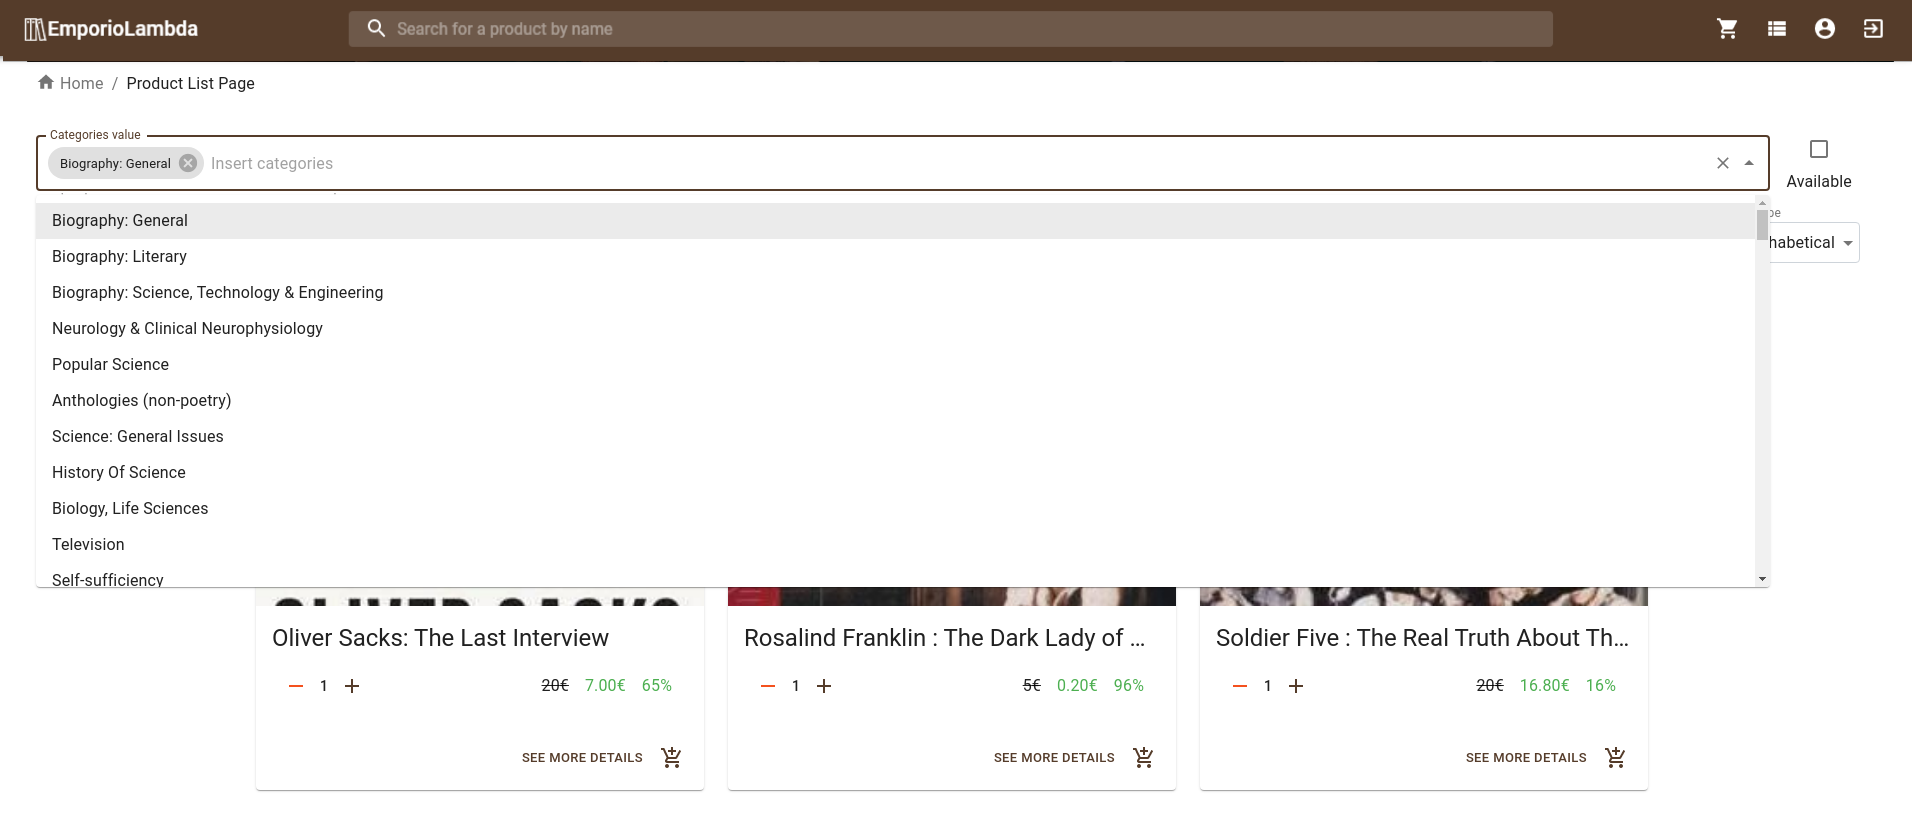
\includegraphics[scale=0.25]{Immagini/Acquirente/plp-categories-open.png}
	\caption{Filtro prodotti per categorie}
	\label{fig:PLPcategorie}
\end{figure}
\subsubsection{Filtro prodotti per disponibilità}
Per visualizzare i prodotti in base alla loro disponibilità, l'utente può selezionare la casella indicata.
\begin{figure}[H]
	\centering
	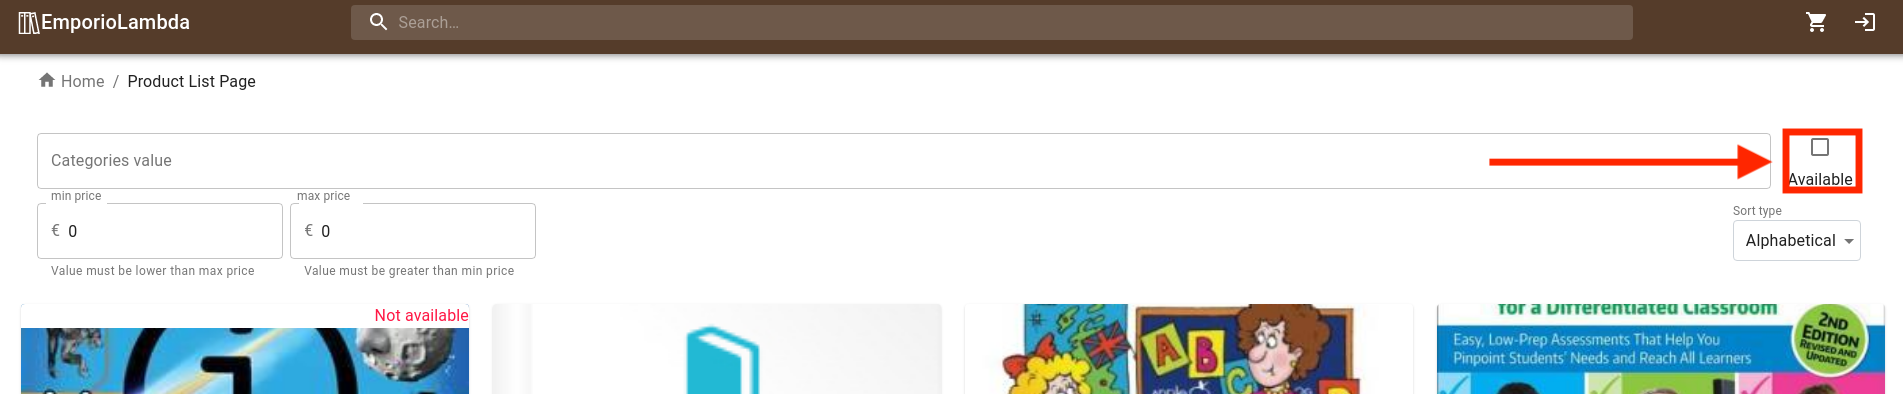
\includegraphics[scale=0.25]{Immagini/Acquirente/plp-available.png}
	\caption{Filtro prodotti per disponibilità}
	\label{fig:PLPdisponibilità}
\end{figure}
\subsubsection{Filtro prodotti per prezzo}
Per visualizzare i prodotti in base al loro prezzo, l'utente può inserire nelle caselle (1) e (2) il valore minimo e massimo per effettuare la ricerca.
\begin{figure}[H]
	\centering
	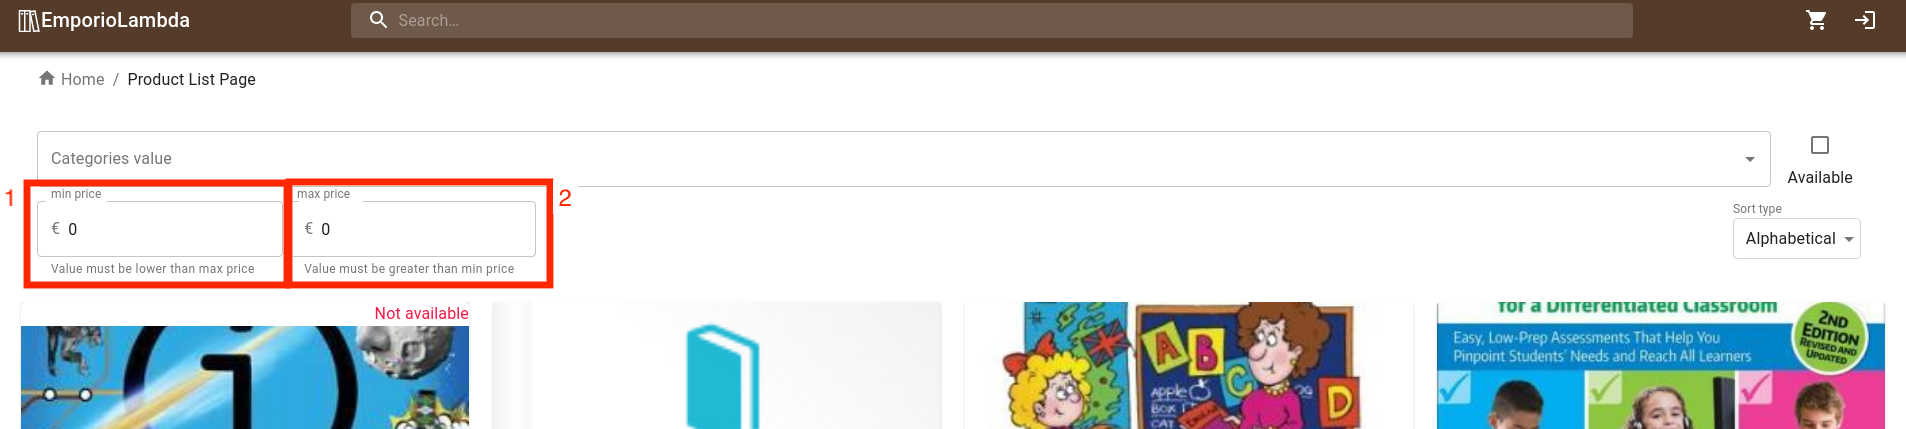
\includegraphics[scale=0.25]{Immagini/Acquirente/plp-price.png}
	\caption{Filtro prodotti per prezzo}
	\label{fig:PLPprezzo}
\end{figure}
\subsection{Visualizzazione del carrello}
Premendo sull'icona del carrello presente in ogni schermata è possibile per l'utente accedere al proprio carrello. Verranno visualizzati oltre ai vari prodotti con le loro informazioni:
\begin{enumerate}
	\item Prezzo totale;
	\item Icona per procedere al pagamento.
\end{enumerate} 
\begin{figure}[H]
	\centering
	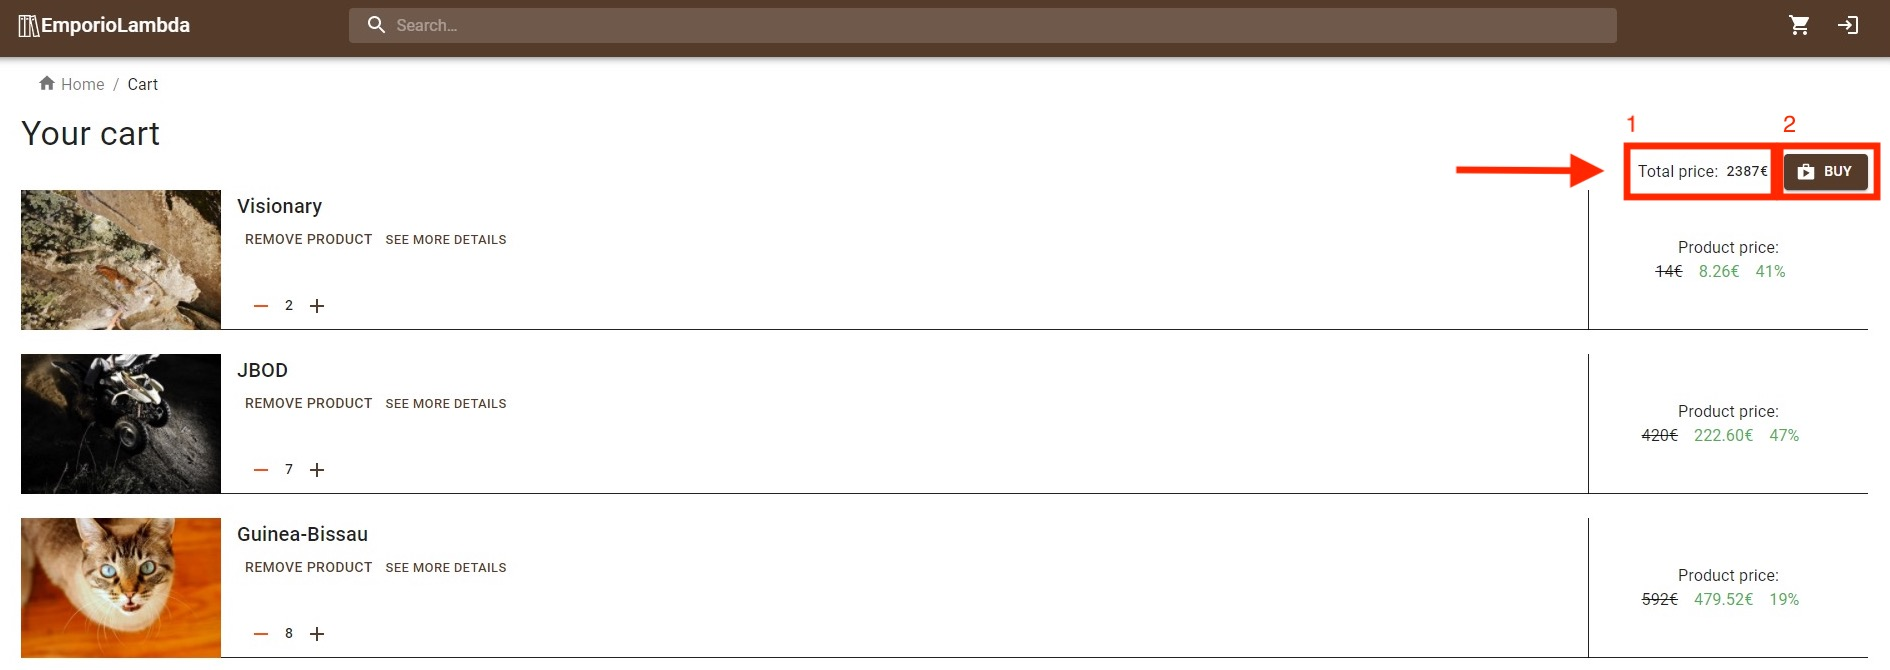
\includegraphics[scale=0.25]{Immagini/Acquirente/Cart.JPG}
	\caption{Carrello}
	\label{fig:Carrello}
\end{figure}
\subsection{Pagamento e gestione della spedizione}
Dopo aver cliccato sull'icona per procedere al pagamento si verrà reindirizzati ad una schermata di riepilogo prima di procedere con l'effettivo checkout.
Nella schermata è possibile visualizzare nuovamente l'elenco dei vari prodotti presenti nel carrello cliccando sull'apposita icona.
\begin{figure}[H]
	\centering
	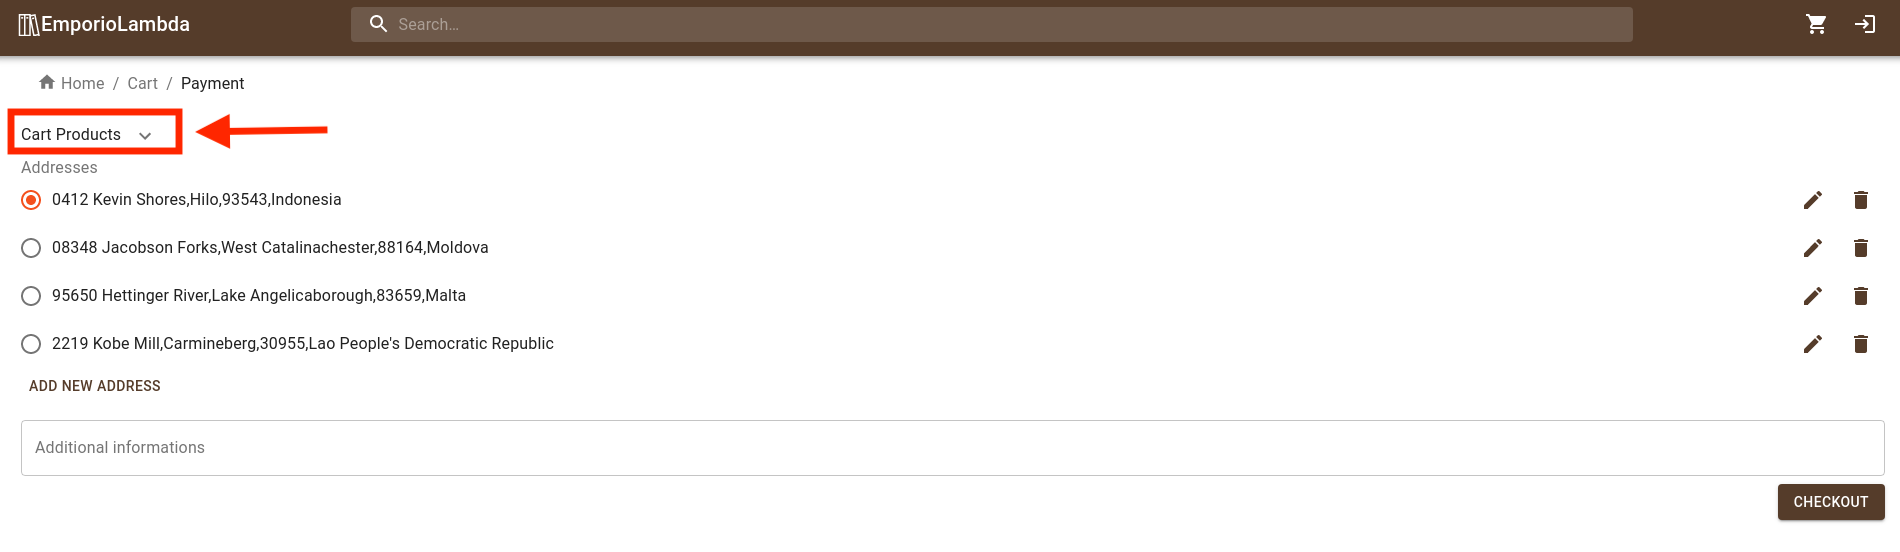
\includegraphics[scale=0.25]{Immagini/Acquirente/payment.cartproduct.png}
	\caption{Schermata di riepilogo prima del checkout}
	\label{fig:CartProduct}
\end{figure}
\begin{figure}[H]
	\centering
	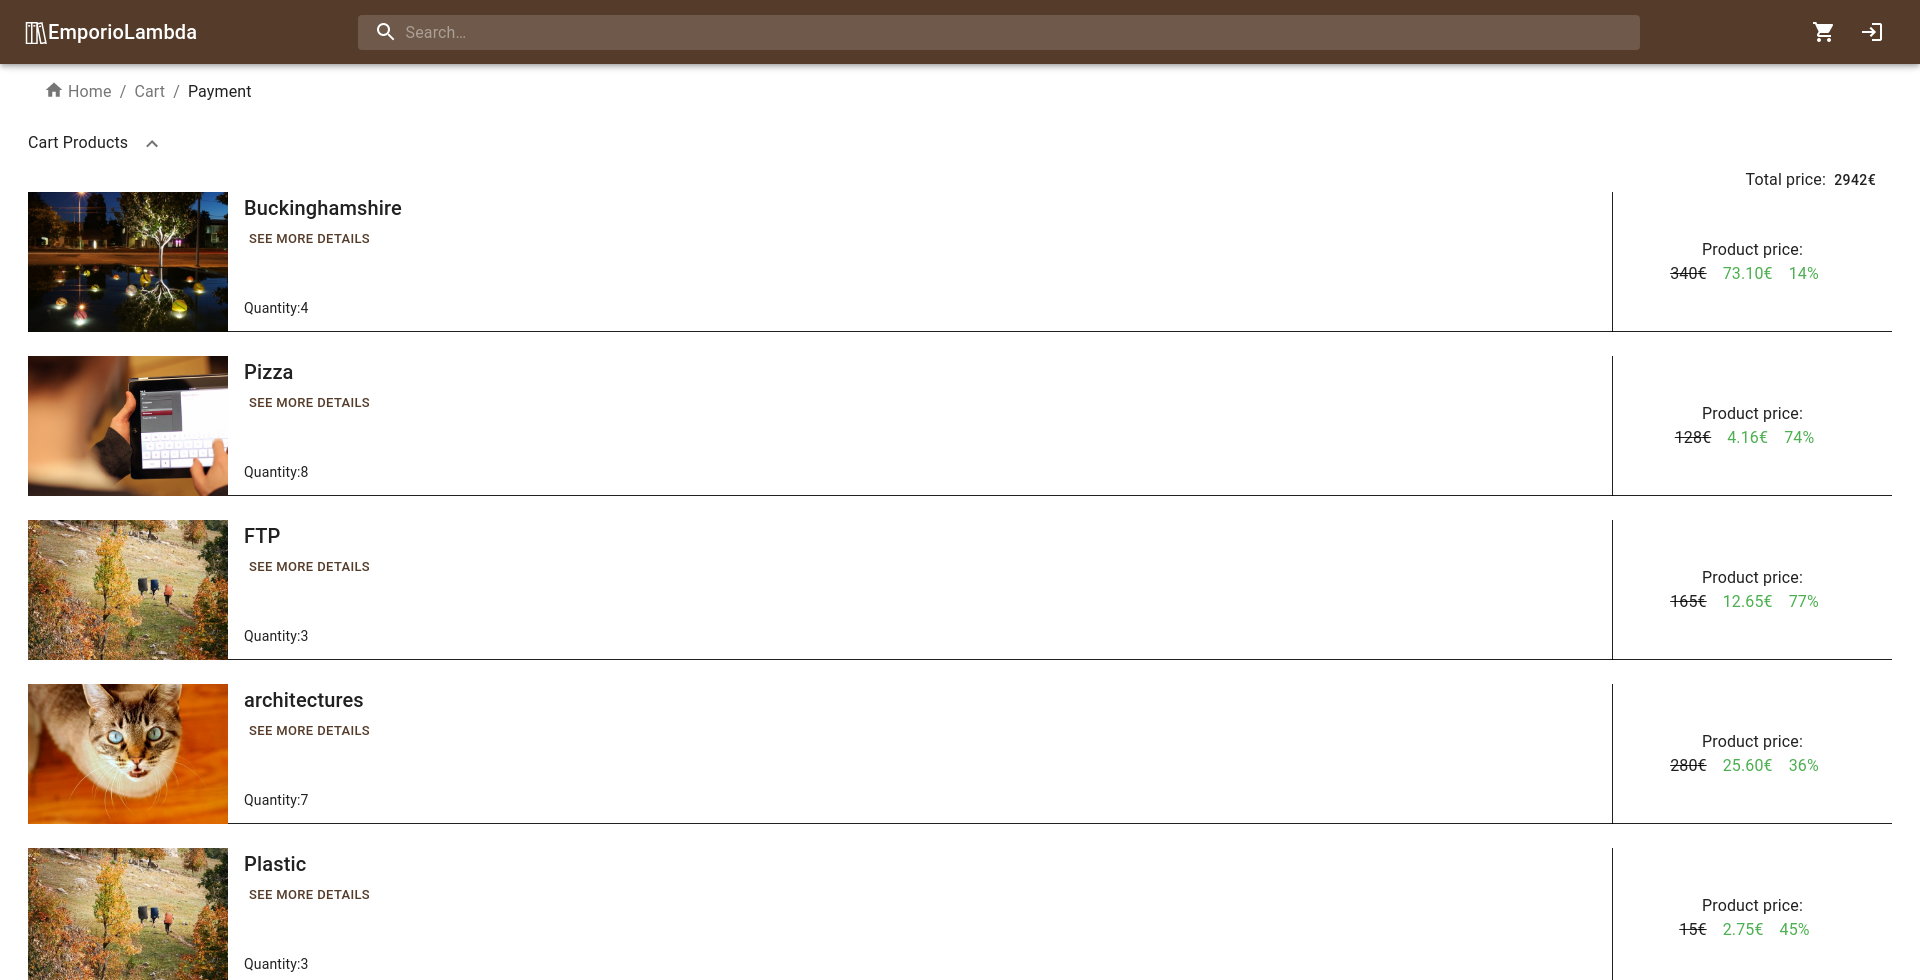
\includegraphics[scale=0.25]{Immagini/Acquirente/payment-products-open.customer.png}
	\caption{Schermata elenco prodotti nel carrello}
	\label{fig:CartProductElenco}
\end{figure}
Potranno essere inserite delle informazioni aggiuntive per il venditore.
\begin{figure}[H]
	\centering
	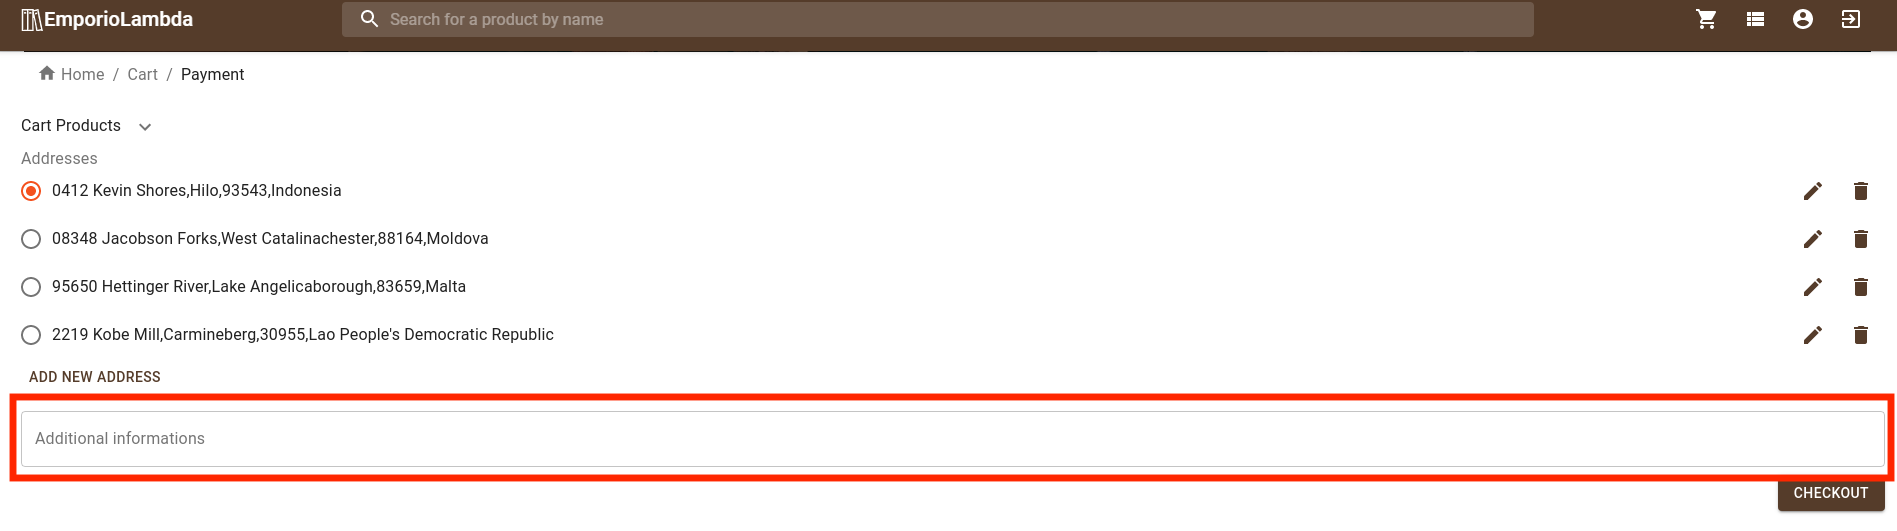
\includegraphics[scale=0.25]{Immagini/Acquirente/payment.addinfo.png}
	\caption{Schermata elenco di riepilogo prima del checkout con \glo{form} per inserimento informazioni aggiuntive}
	\label{fig:CartAddinfo}
\end{figure}
Nella stessa schermata sarà possibile gestire gli indirizzi di spedizione precedentemente inseriti, inserirne uno nuovo e selezionare l'indirizzo prescelto per l'ordine.
\begin{figure}[H]
	\centering
	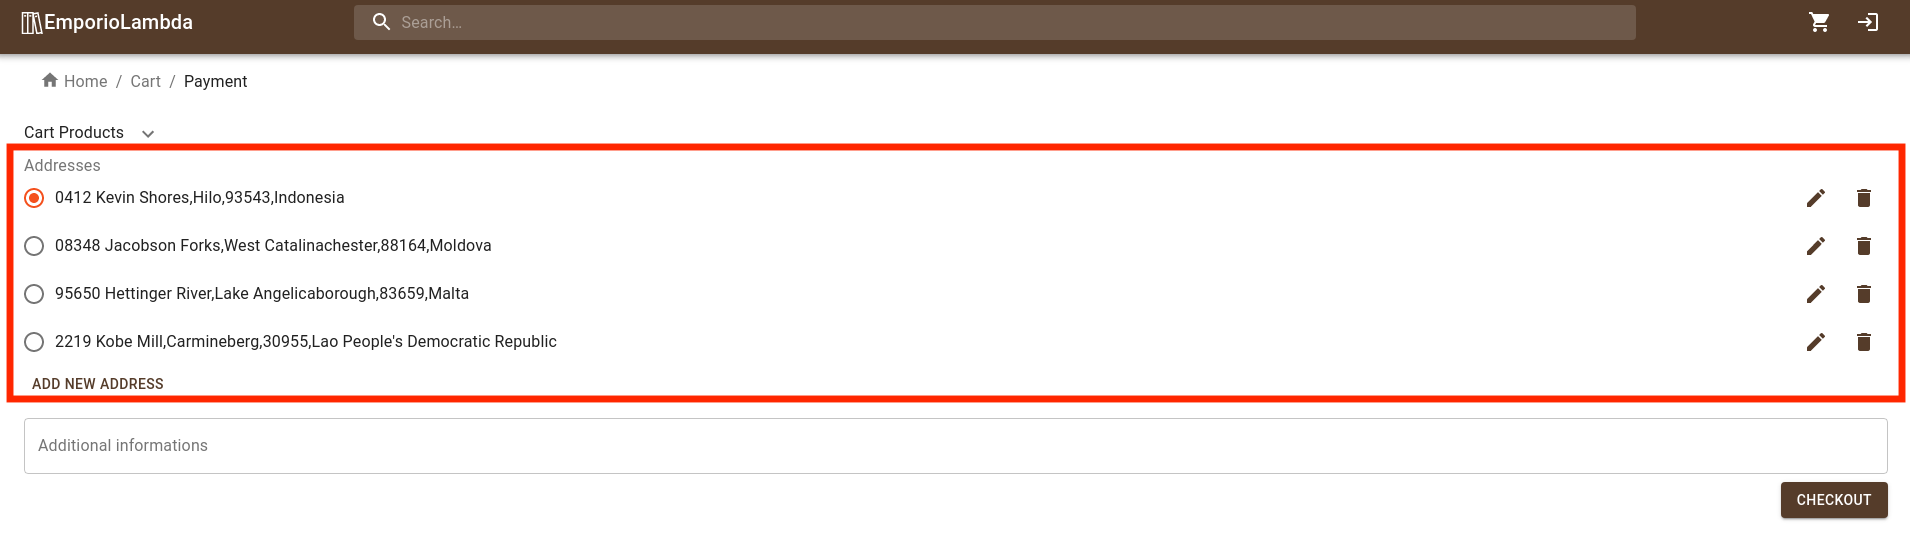
\includegraphics[scale=0.25]{Immagini/Acquirente/payment.customer.png}
	\caption{Schermata di riepilogo prima del checkout in cui gestire gli indirizzi}
	\label{fig:CartAddress}
\end{figure}
\subsubsection{Inserimento nuovo indirizzo}
Per inserire un nuovo indirizzo l'utente deve premere sulla scritta apposita, apparirà un \glo{form} in cui potrà inserire i vari dati relativi al nuovo indirizzo.
\begin{figure}[H]
	\centering
	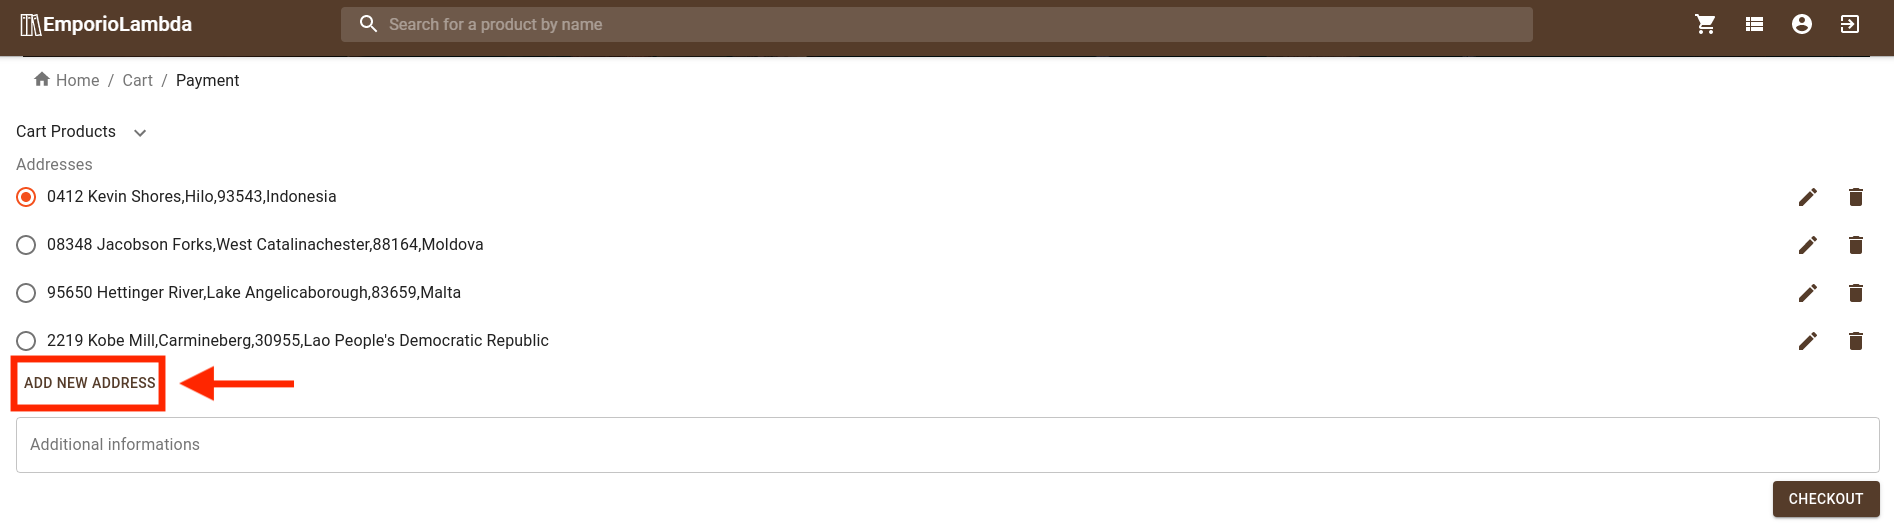
\includegraphics[scale=0.25]{Immagini/Acquirente/payment.addressnew.png}
	\caption{Schermata di riepilogo prima del checkout per inserire nuovo indirizzo}
	\label{fig:NewAddress}
\end{figure}
\begin{figure}[H]
	\centering
	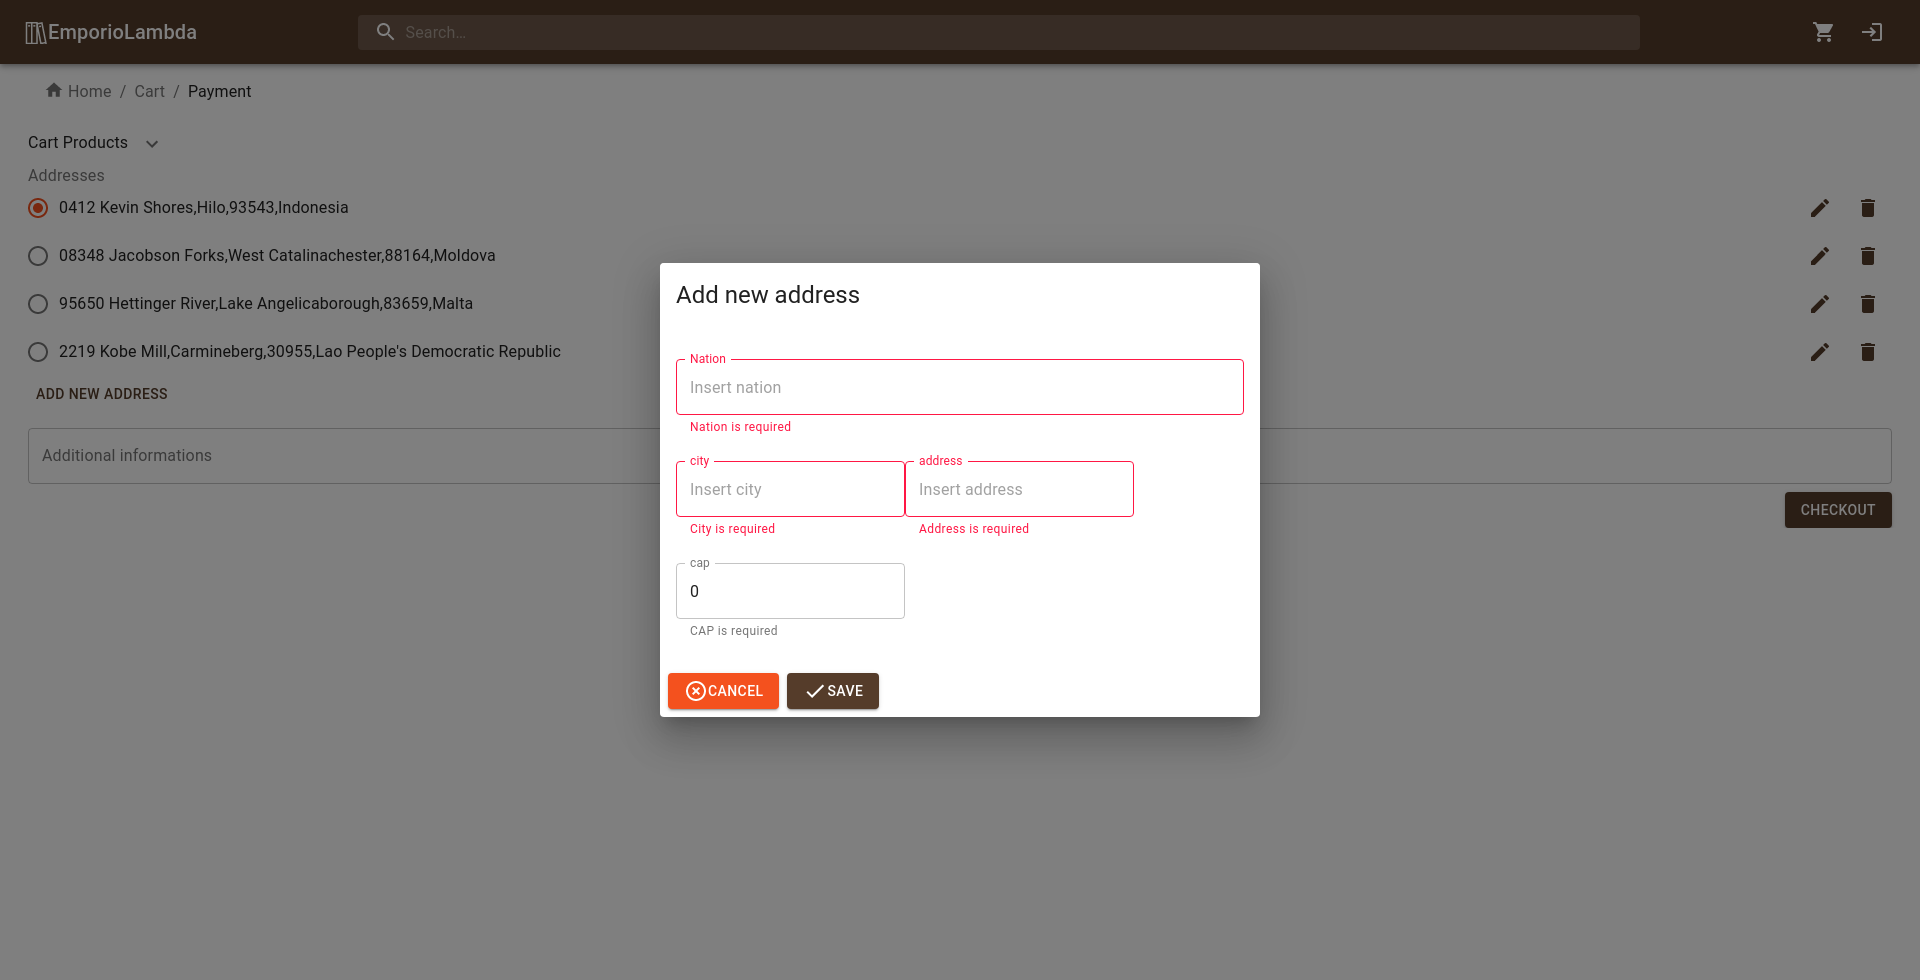
\includegraphics[scale=0.25]{Immagini/Acquirente/payment-new-address.customer.png}
	\caption{Form di inserimento nuovo indirizzo}
	\label{fig:CartnewAddress}
\end{figure}
\subsubsection{Eliminazione di un indirizzo inserito precedentemente}
Per eliminare un indirizzo precedentemente inserito l'utente deve cliccare sull'icona del cestino e confermare l'eliminazione.
\begin{figure}[H]
	\centering
	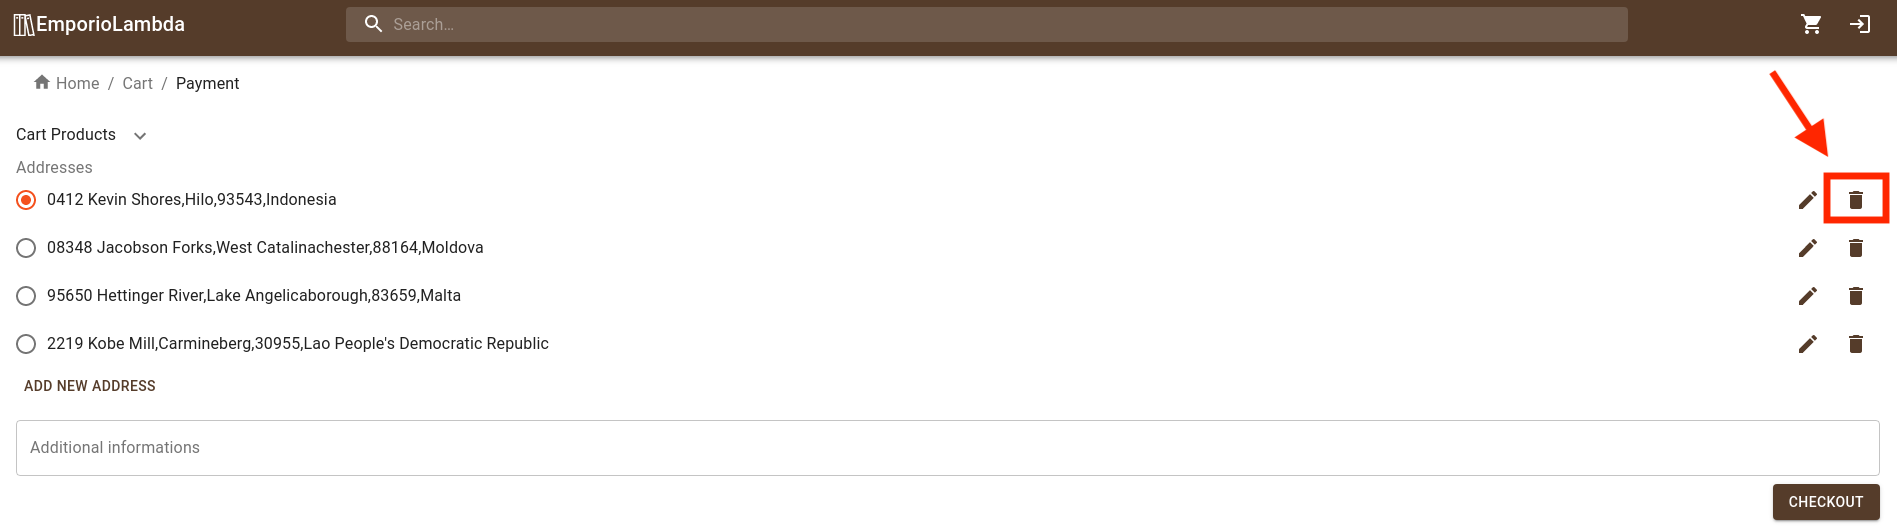
\includegraphics[scale=0.25]{Immagini/Acquirente/payment.addressdelete.png}
	\caption{Schermata di riepilogo prima del checkout per eliminare un indirizzo}
	\label{fig:DeleteAddress}
\end{figure}
\begin{figure}[H]
	\centering
	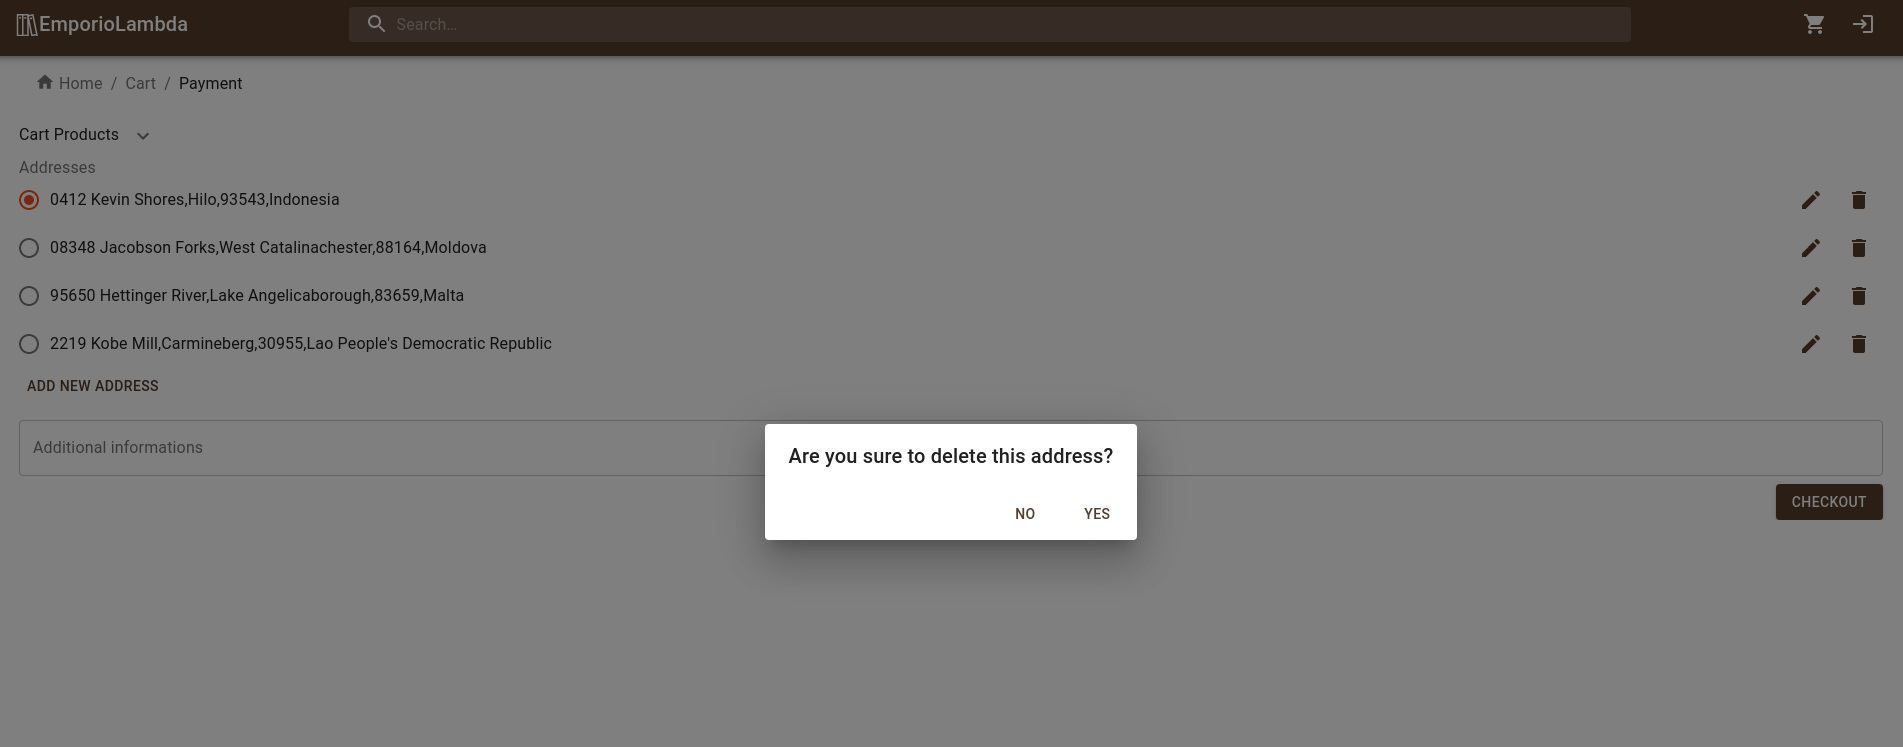
\includegraphics[scale=0.25]{Immagini/Acquirente/payment-delete-address.customer.png}
	\caption{Form di conferma eliminazione indirizzo}
	\label{fig:CartDeleteAddress}
\end{figure}
\subsubsection{Modifica di indirizzo inserito precedentemente}
Per modificare un indirizzo precedentemente inserito l'utente deve cliccare sull'icona della penna, si aprirà il form per modificare l'indirizzo.
\begin{figure}[H]
	\centering
	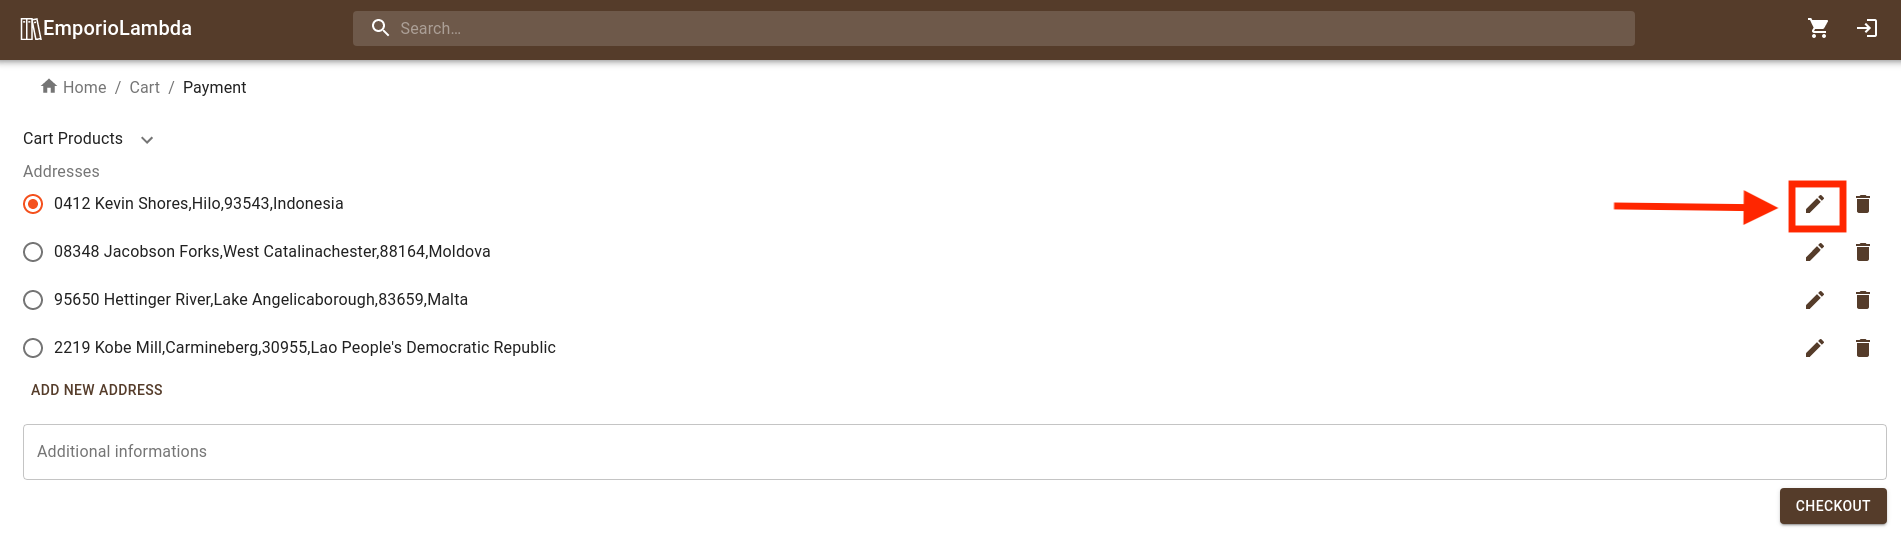
\includegraphics[scale=0.25]{Immagini/Acquirente/payment.addressmodify.png}
	\caption{Schermata di riepilogo prima del checkout per modificare un indirizzo}
	\label{fig:EditAddress}
\end{figure}
\begin{figure}[H]
	\centering
	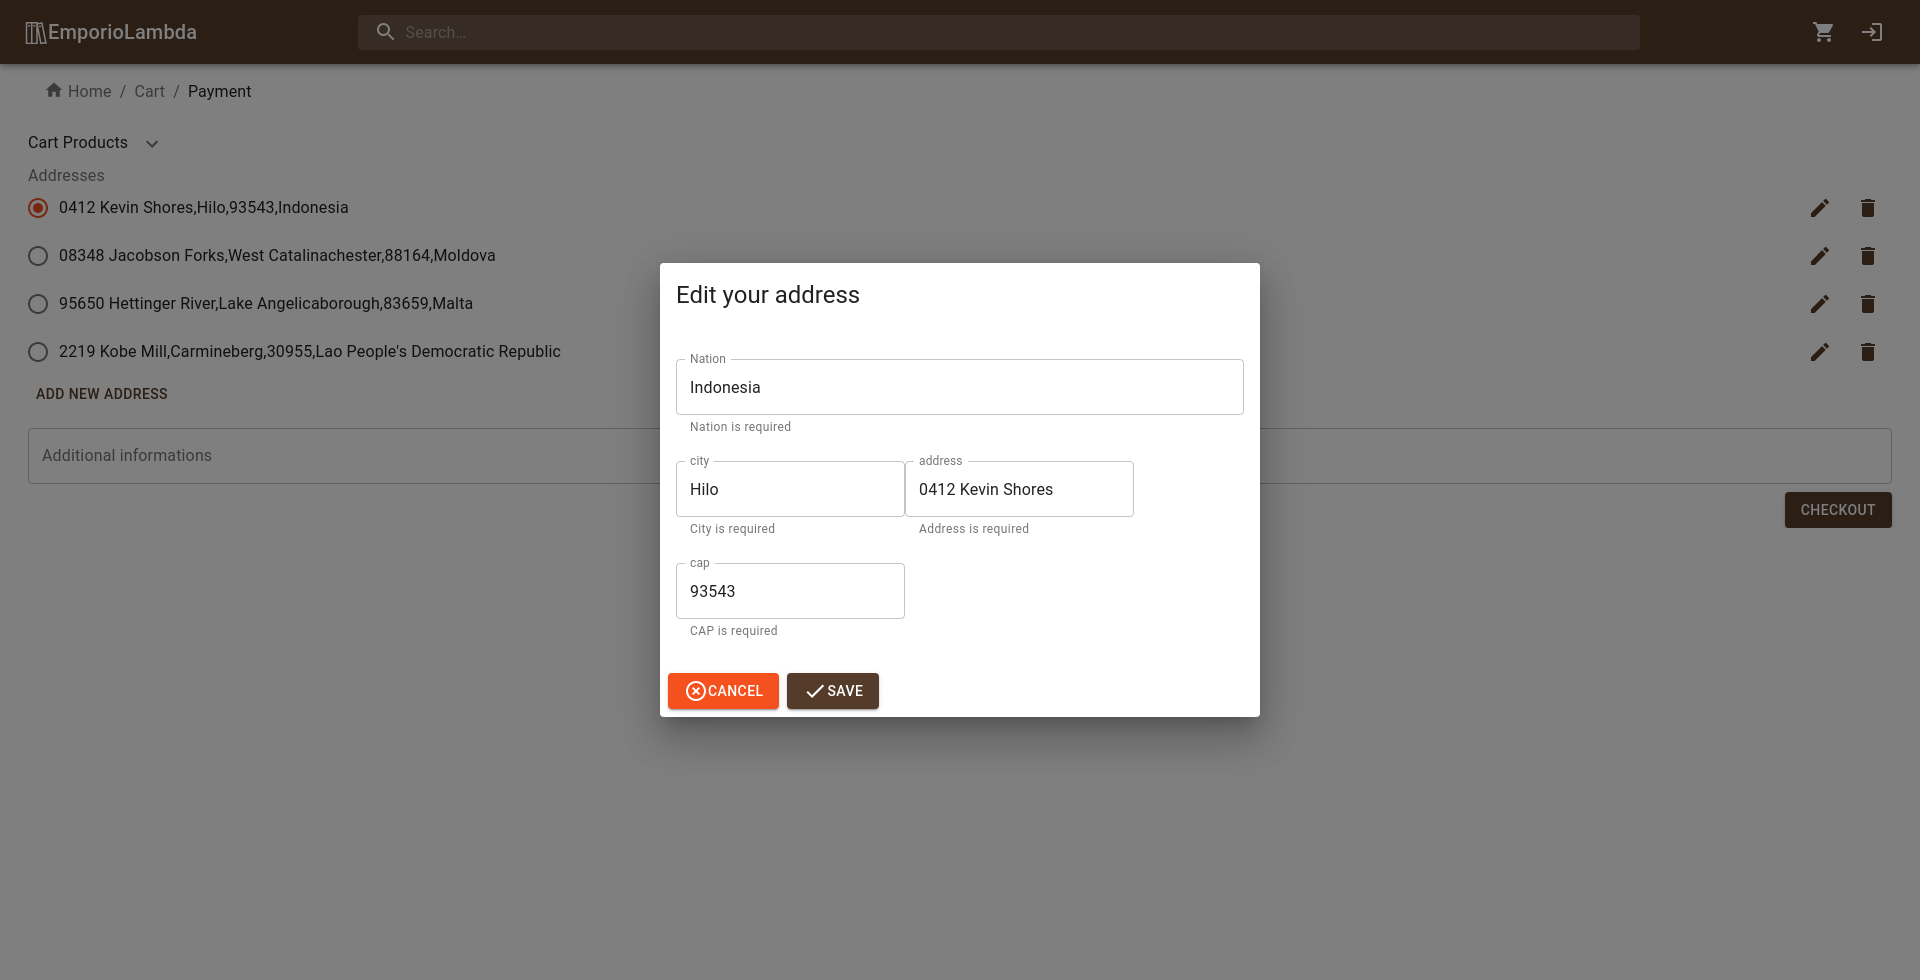
\includegraphics[scale=0.25]{Immagini/Acquirente/payment-edit-address.customer.png}
	\caption{Form per modificare l'indirizzo}
	\label{fig:CartEditAddress}
\end{figure}
\subsubsection{Procedere con il checkout}
Per procedere con il pagamento è necessario cliccare sull'apposito bottone, l'utente verrà reindirizzato alla schermata in cui inserire i dati per il pagamento e completare l'ordine.
\begin{figure}[H]
	\centering
	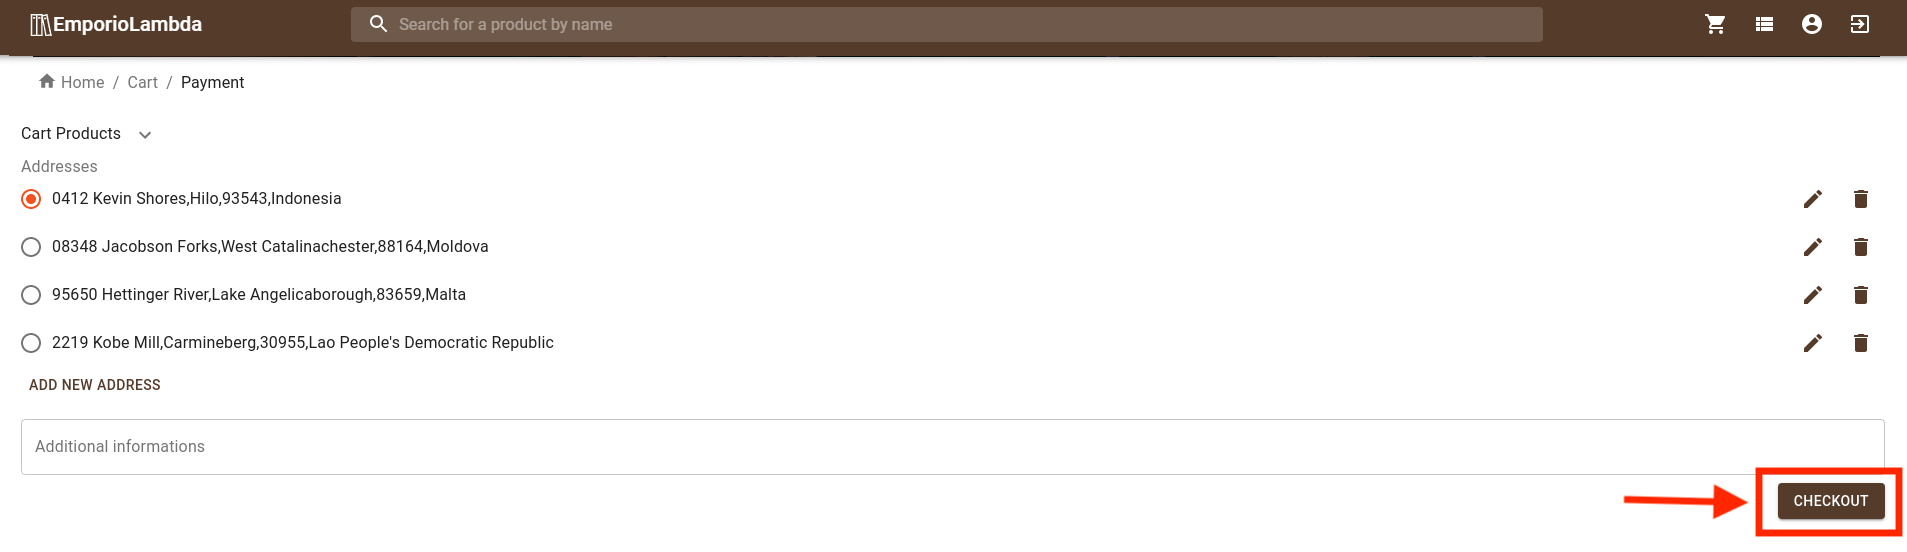
\includegraphics[scale=0.25]{Immagini/Acquirente/payment.checkout.png}
	\caption{Schermata di riepilogo prima del checkout con icona per procedere con il pagamento}
	\label{fig:CartCheckout}
\end{figure}